\begin{figure}[ht]
    \centering
    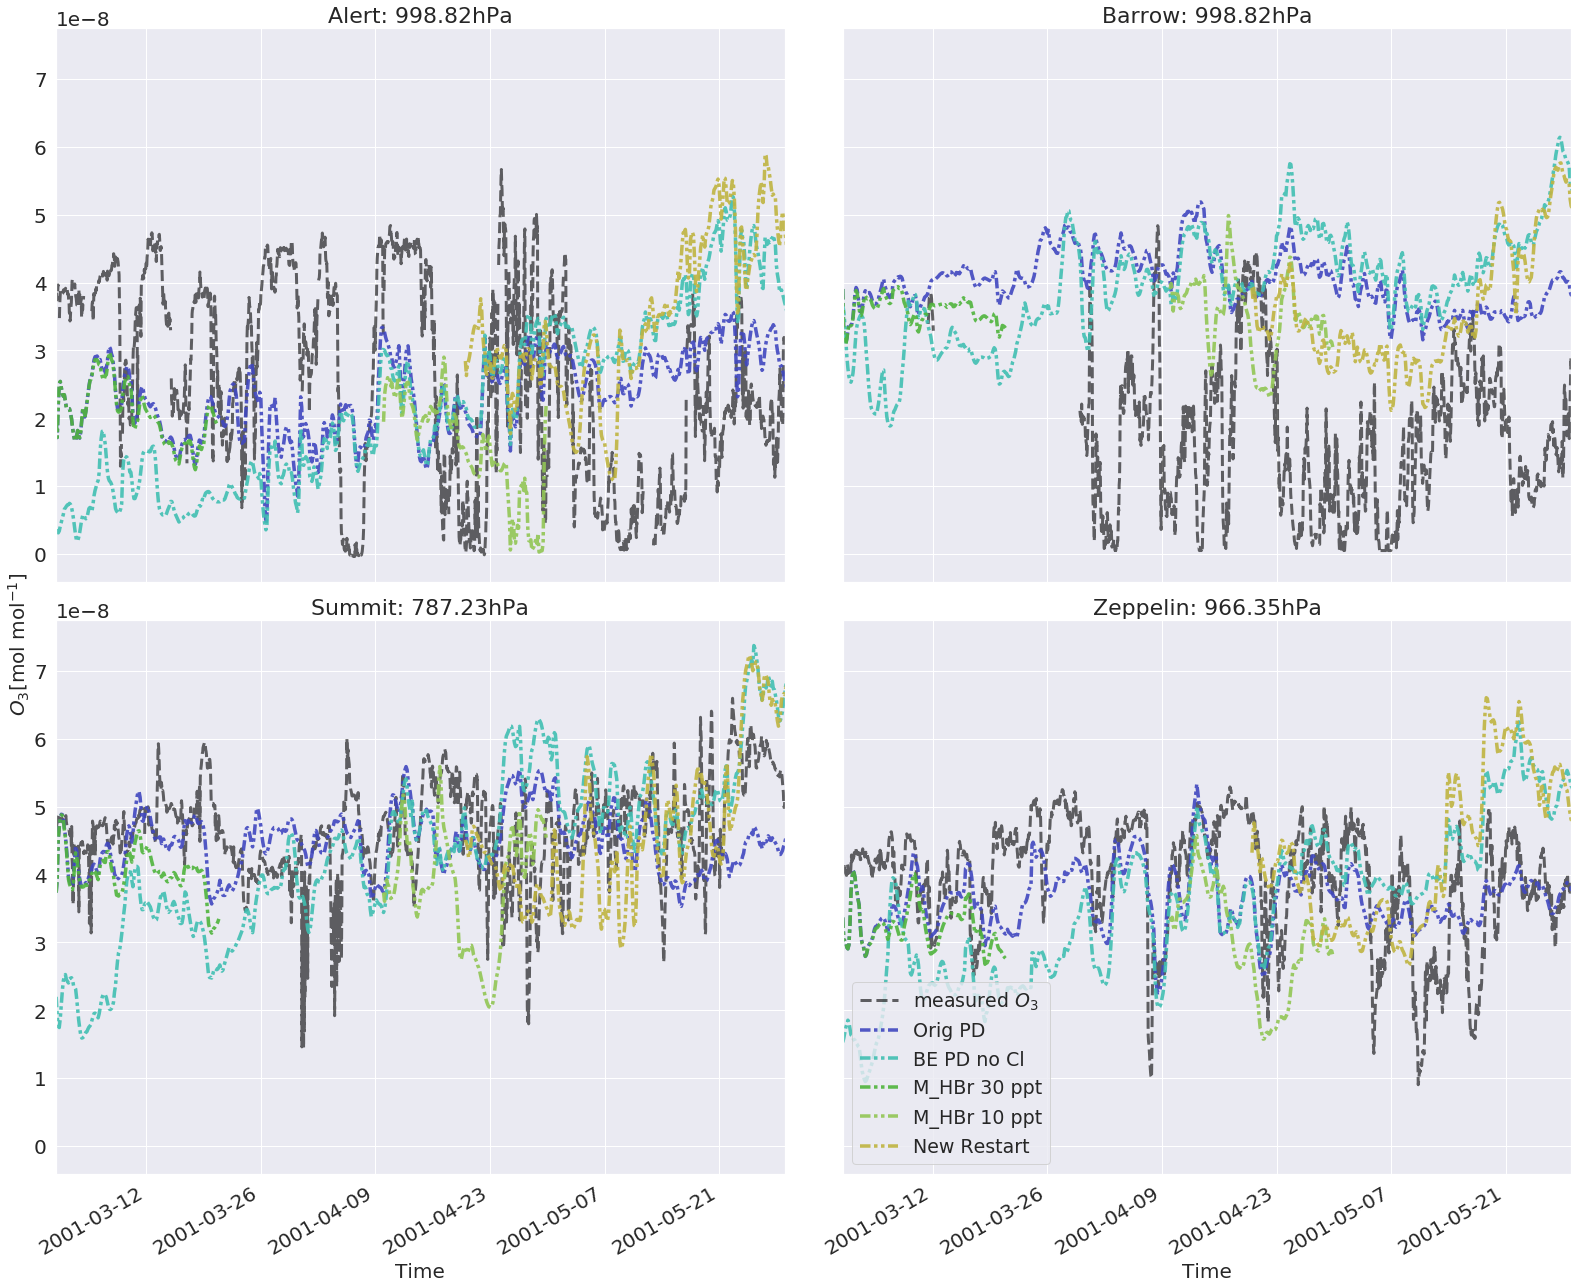
\includegraphics[width=\linewidth]{Chapter6_Results/images/ozone_noCl_step2.png}
    \caption{Ozone measurements (black line) and model results from the original CTM3 (blue line), Branch \ref{def:BE_PD_noCl} (turquoise line) (these three are the same as in Figure \ref{fig:test_RemoveHetReacts}), Branch \ref{def:BE_PD_noCl} with hard coded \chem{HBr}-concentration of 30 ppt (green line), Branch \ref{def:BE_PD_noCl} with hard coded \chem{HBr}-concentration of 10 ppt(light green line) and Branch \ref{def:BE_PD_noCl} initialized with a restart file from the hard coded \chem{HBr}-concentration of 10 ppt- run (yellow line) at the four different stations, Alert (top left), Barrow (top right), Summit (lower left) and Zeppelin (lower right) with available measurements in 2001. Model results are taken from the first model level at $998.82 hPa$. PD = present day, BE = bromine explosion}
    \label{fig:ozone_noCl_step2}
\end{figure}